%!TEX root=paper.tex

\section{System Overview}

\clue is a metric-centric provenance and simulation system that helps users
understand how complex dashboard metrics are derived and how changes in
underlying data affect the final metric value. Therefore, the system should be
able to (1)~extract and represent metrics from transformation pipelines,
(2)~generate actionable suggestions for how to achieve a target metric change
through data manipulation. However, these requirements pose several challenges:
(1)~the system must handle complex transformation steps into meaningful metric
relationships even though the transformation logic that did not explicitly
define metrics. (2)~it must generate meaningful suggestions that are relevant to
the user's target and grounded in the data in real-time. The possible
suggestions are combinatorial in nature, hence the system must efficiently
search and rank them to present the most useful options.

\noindent \textbf{Metric Provenance Graph}. \clue maintains a metric provenance
graph for interactive explanation and simulation of complex metrics. The graph
is modeled as a bipartite graph consisting of Metric nodes and Computation-Rule
nodes. Each Metric node is associated with a rule node that encodes how it is
computed (e.g., sum, ratio, product, average), while rule nodes connect to their
input Metric nodes via directed edges, representing the computation used to
derive the parent metric from its children. In the \metric{PLTV} example,
\metric{PLTV}, \metric{Probability of Active}, \metric{Expected Number of
Orders}, and \metric{expected\_order\_value} are all represented as Metric
nodes. The \metric{PLTV} node is connected to a product-rule node via a directed
edge,  and the rule node is also linked to the three input metrics, indicating
that $\metric{PLTV} = \metric{Probability of Active}  \times \metric{Expected
Number of Orders} \times \metric{expected\_order\_value} $

Similarly, for the transformation T99 in the left of Figure~\ref{tab:metrics},
an average-rule node connects the input metrics \metric{\#\_orders} and
\metric{\#\_total\_gross\_value} to the output metric \metric{expected\_order
\_value}. 

\noindent \textbf{Data Transformation Graph}. Underneath the metric provenance
graph, \clue also constructs the data transformation graph from SQL-based
pipelines. We leverage a SQL parsing framework, SQLGlot~\cite{sqlglot}, to
convert each query into an abstract syntax tree (AST), from which we identify
source tables, intermediate operations, and output columns. Column-level lineage
is then resolved by tracing how each output column is derived from upstream
columns across CTEs, subqueries, and joins. The resulting graph models
transformations as a directed graph, where nodes represent columns and
operations, and edges encode ``derived-from'' relationships with operation types
such as aggregation, arithmetic computation, filtering, and joins. 

Within this graph, a Column node is considered a metric or submetric candidate
if it (i)~is numeric and (ii)~is derived through aggregation or arithmetic
expressions. For instance, columns such as \texttt{\#\_orders} (from a COUNT
aggregation), \texttt{gross\_value} (from SELECT(revenue - cost)), and
\texttt{expected\_order\_value} are valid candidates. In contrast, raw
attributes (e.g., order\_id, subtotal) or derived boolean flags do not qualify.

\noindent \textbf{Connecting the Two Graphs}. When a metric is derived from a
concrete data-table operation, CLUE connects the corresponding Metric node in
the metric provenance graph to a Column node in the data transformation graph
through a BACKED\_BY edge. For example, the Metric node \texttt{\#\_total
\_gross\_value} created based on T98 is associated with the Column node
\texttt{gross\_value}, which is derived from the SQL expression SELECT (revenue
- cost) in T97. Through this linkage, CLUE enables users to move seamlessly from
high-level metric explanations to the underlying data transformations that
produce them. The unified graph, including both the data provenance and the
metric graph, is serialized in JSON format and imported into a Neo4j graph
database for efficient querying.

\noindent \textbf{Metric Explanation Generator.} To make the system accessible
to non-technical users, \clue includes an explanation layer that translates both
provenance and simulation results into natural language descriptions using
GPT-5.4 model. For provenance, \clue explains how a metric is composed from
submetrics. For simulation, it summarizes the old and new values of affected
nodes, and describes the propagation path of the change through the graph. In
the example above, \clue present the explanation: ``Increasing \texttt{\#\_total
\_gross\_value} by 200 raises \texttt{expected\_order\_value} from 25 to 30,
which increases \texttt{PLTV} from 10 to 12.''

\noindent \textbf{Data Manipulation Suggestions.} Given a user-specified target
change for a metric and the metric provenance graph, \clue aims to generate data
manipulation suggestions to help user reason how changes in underlying data can
achieve the desired metric outcome. To achieve this, \clue first locates the
selected metric node in the metric layer and traverses its dependency structure
to identify upstream submetrics and values on the leaf nodes. Next, it generates
suggestions from a set of adjustment strategies, such as changing the value of a
single component, distributing changes across multiple components, increasing a
numerator or denominator in a ratio, shifting an average by adding high or low
value records. These templates are not domain-specific actions, but abstract
intervention operators defined over the metric graph, such as ADD, SUB, SET, or
SCALE on leaf quantities. This design allows the same suggestion generation
mechanism to be reused across domains, while the meaning of each intervention is
grounded in the graph structure and the labels of the affected nodes.

For each adjustment strategy, \clue instantiates candidate suggestions by
solving for the leaf-level changes required to move the selected metric toward
the user's target. Continuing the example of the \metric{PLTV} metric, assuming
the current value of \metric{PLTV} is 10 and the target is 12, \clue derives a
candidate suggestion that increases \metric{\#\_total \_gross\_value} by 200
since this raises \metric{expected\_order\_value} from 25 to 30 and yields the
desired increase in \metric{PLTV}.

Next, all feasible suggestions are ranked using a combination of criteria,
including (i)~\textbf{minimal target overshoot}
% \wc{why we don't make the
% candidate be close to the target in the first place?} ~\ew{The suggestion
% generator supposes to produce a set of feasible suggestions that satisfy the
% user’s goal at least minimally. Is this what you thought of?}
, favoring candidates whose simulated outcome meets the user-specified target
with less overshoot; (ii)~\textbf{plausibility}, measured by whether the updated
values remain within semantically valid bounds, such as non-negative counts,
probabilities bounded in $[0, 1]$, or value ranges estimated from percentiles or
$mean \pm 2\sigma$; and (iii)~\textbf{interpretability}, modeled as a proxy for
how easy a recommendation is for users to mentally follow through the metric
graph. Inspired by prior work on explanation complexity and human-simulability
~\cite{lage2019human}, CLUE favors suggestions that modify fewer leaf nodes,
propagate through fewer intermediate nodes, and avoid reuse of the same changed
node across multiple paths of the metric graph. 
% \ew{Added explanation and a citation about how the interpretability of a
% suggestion is measured.} 
After ranking, \clue translates the highest-ranked candidates into natural
language by using the affected metric nodes, operation types. For instance, a
suggestion ``increasing leaf node by 200'' may be rendered as ``Increase total
gross value by 200.'' In this way, \clue combines domain-general suggestion
logic with metric-aware explanations that are understandable to non-technical
users.

\begin{figure*}[t]
    \centering
    \begin{minipage}{0.4975\textwidth}
        \centering
        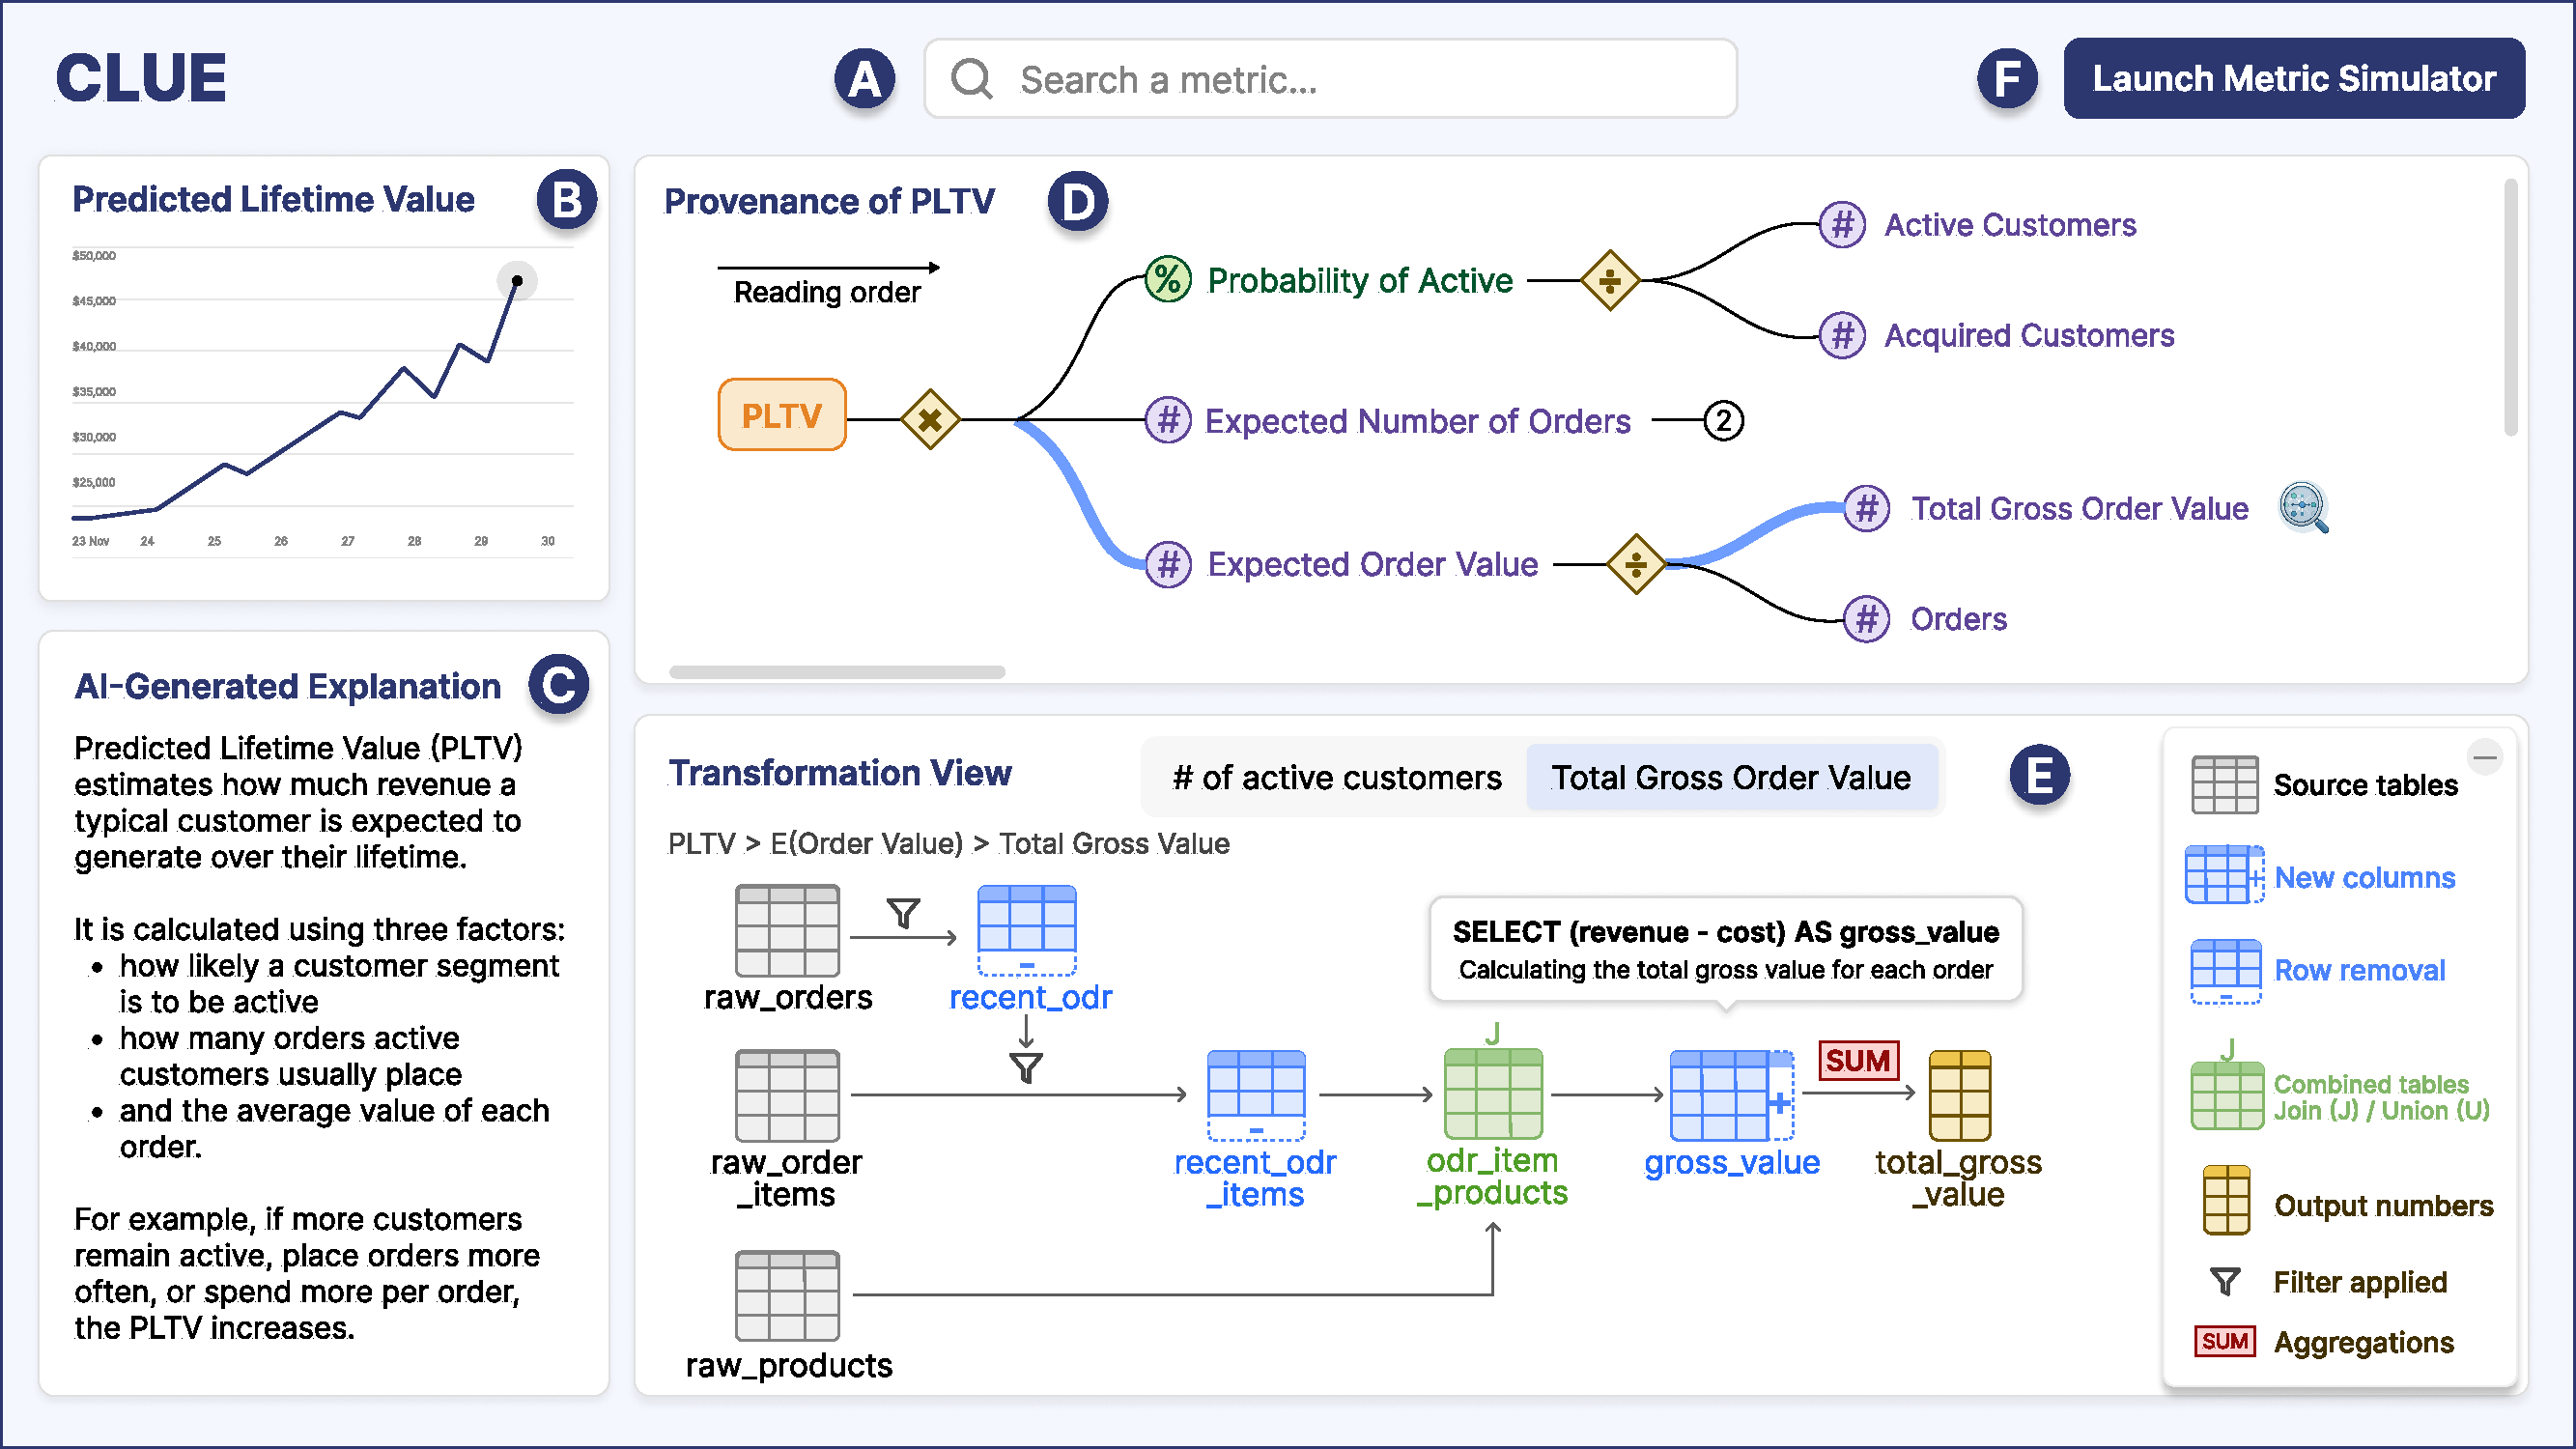
\includegraphics[width=\textwidth,page=1]{figures/UI Wireframe - metric provenance.pdf}
    \end{minipage}
    \hfill
    \begin{minipage}{0.4975\textwidth}
        \centering
        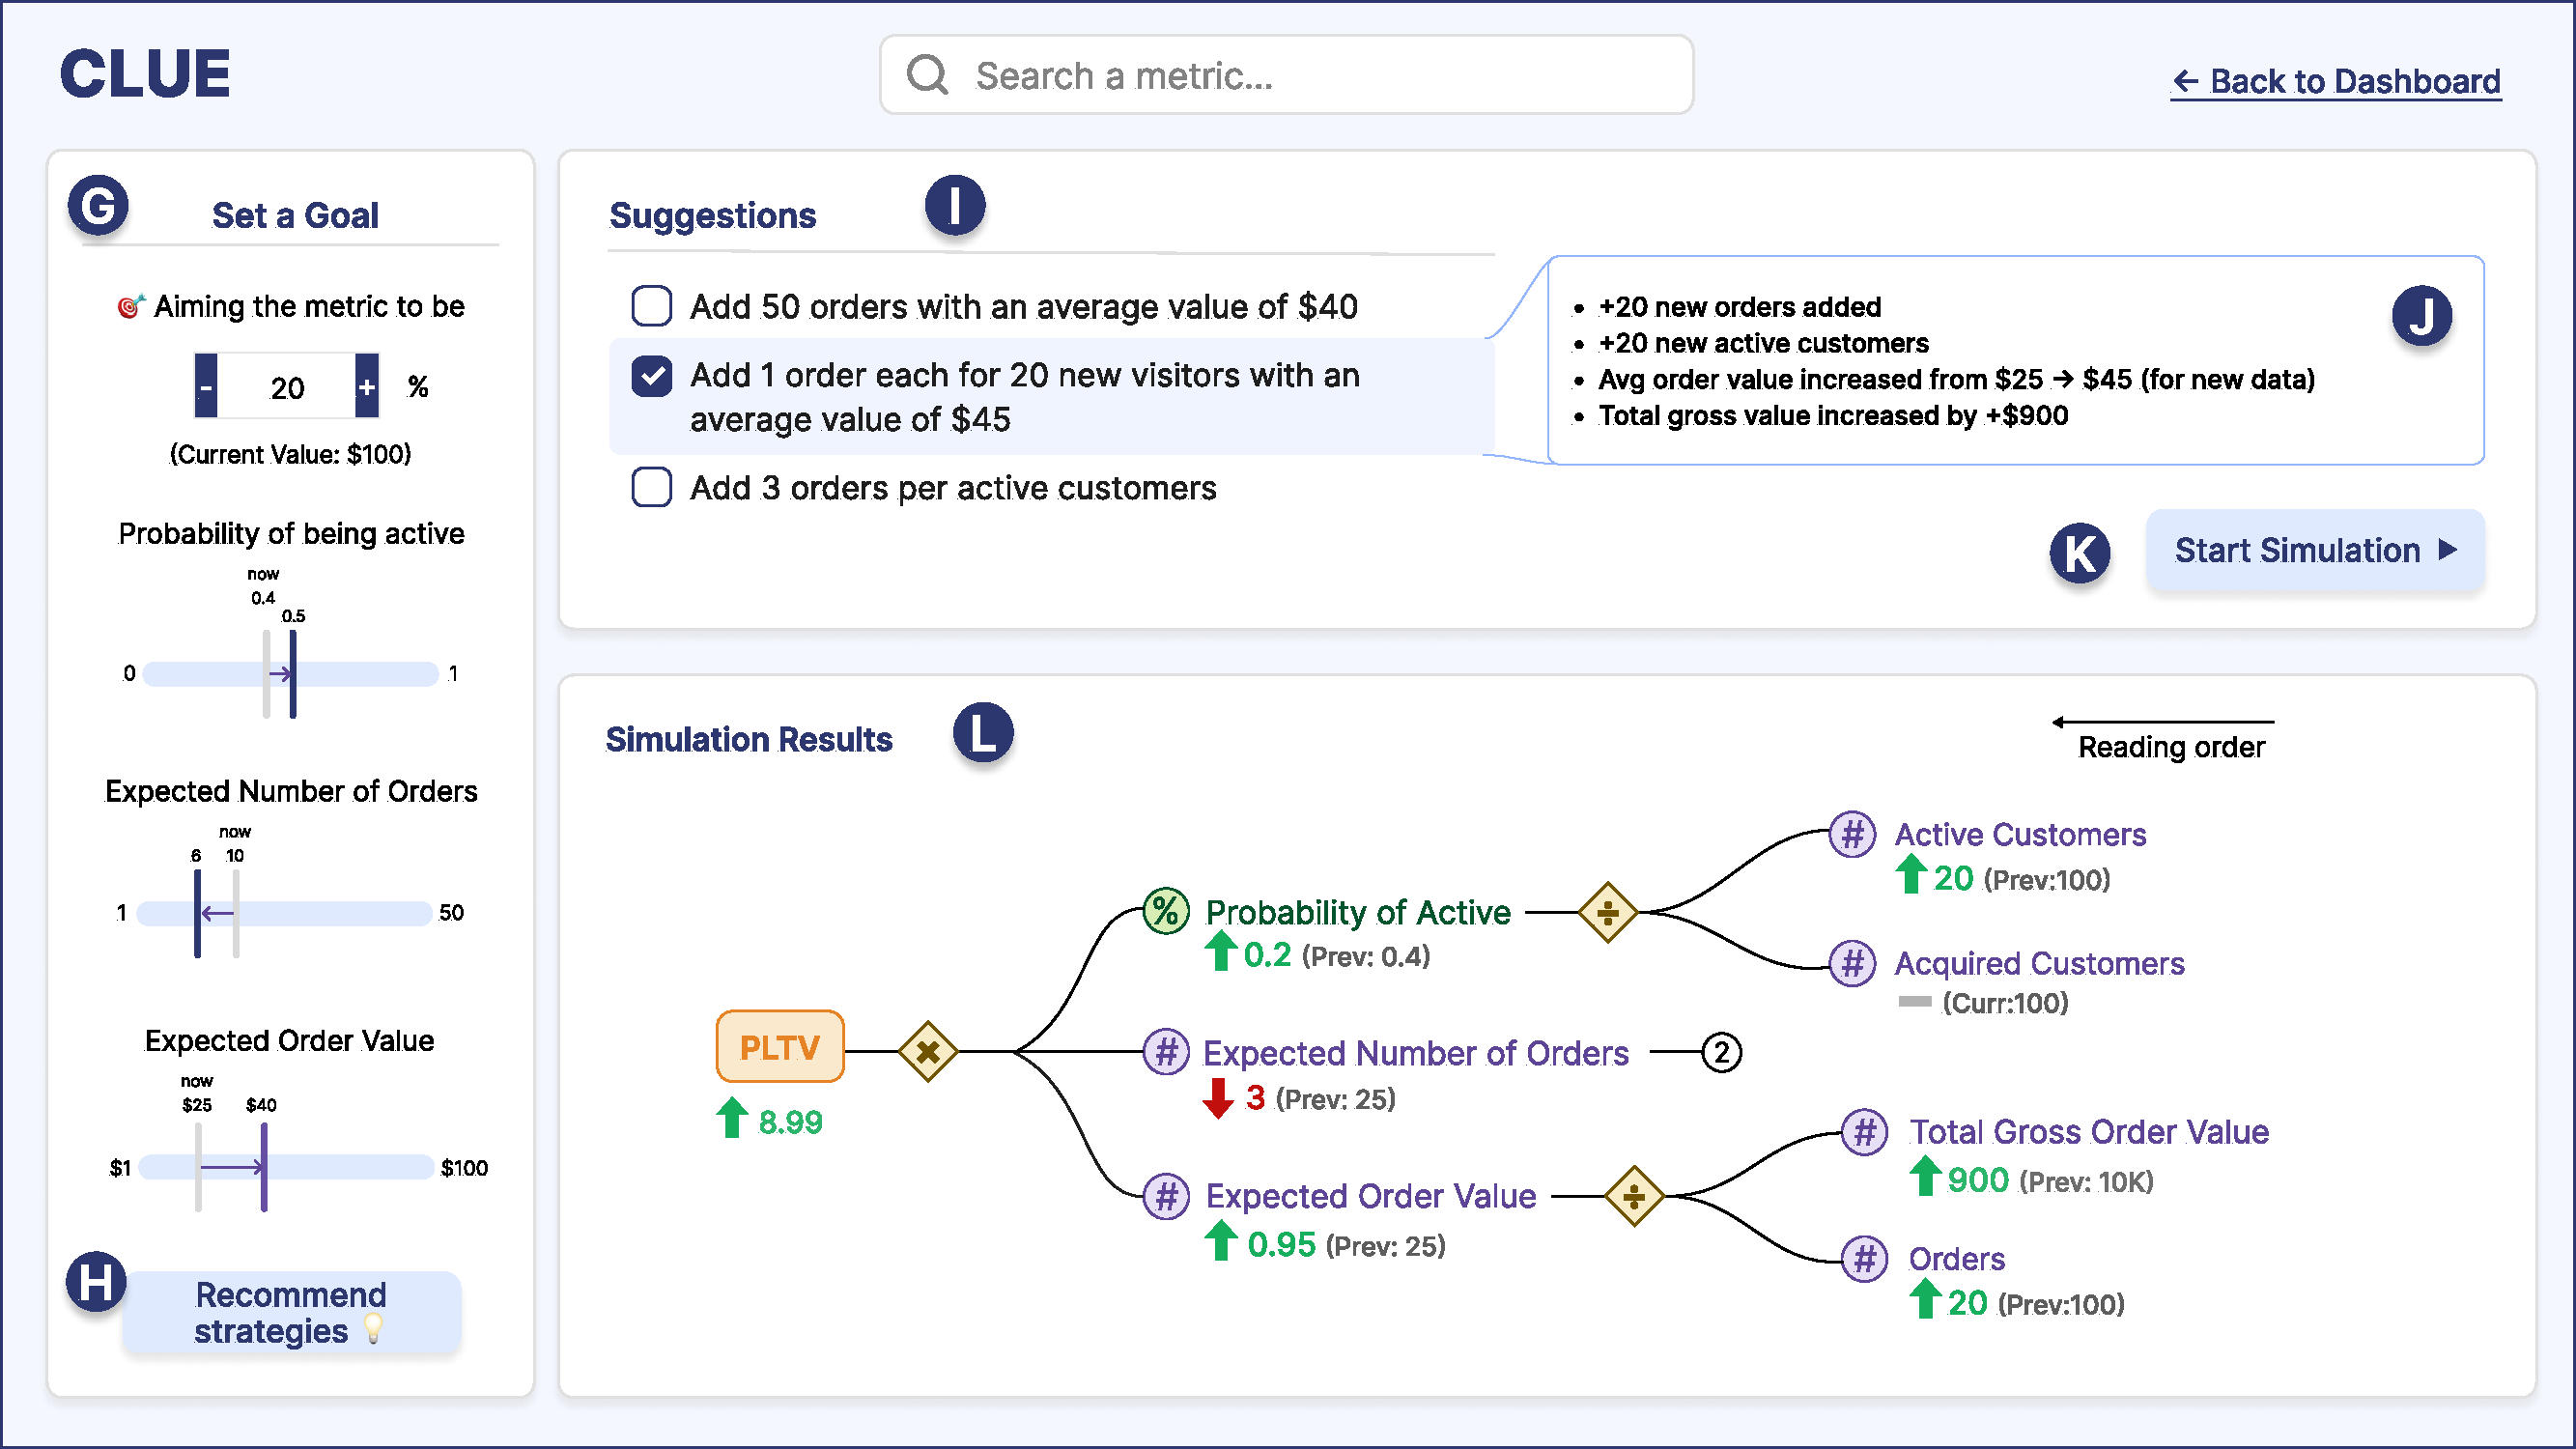
\includegraphics[width=\textwidth,page=1]{figures/UI Wireframe - metric simulator.pdf}
    \end{minipage}
    % 
\includegraphics[width=1\linewidth]{VLDB 2026 Demo//figures/UI Wireframe - metric provenance.pdf}

    {\scriptsize sample scriptsize text}
    \caption{
	\small
	The \clue interface:
    \stepCounter{A} search for a metric, 
    \stepCounter{B} CLUE presents the trend of the metric,
    \stepCounter{C} CLUE generates metric explanation,
    \stepCounter{D} CLUE extracts and visualize metric lineages,
    \stepCounter{E} CLUE extracts and visualize data transformation processes,
    \stepCounter{F} launch the Metric Simulator,
    \stepCounter{G} set up a target number of the metric and tune the desired number for each first-level submetrics,
    \stepCounter{H} generate suggestions to achieve the goal,
    \stepCounter{I} view and select a suggestion, \stepCounter{J} view the data adjustment summary,
    \stepCounter{J} start simulation,
    \stepCounter{K} CLUE computes and presents the value changes on each metric.
    }
\label{clue}
\end{figure*}

\noindent \textbf{Incremental Simulation Engine.} Once a user selects a
suggestion, \clue invokes a simulation engine to apply the selected option to
the live metric value. The engine first updates the affected leaf values, then
traverses the dependency graph upward to identify all ancestor nodes that depend
on the modified leaves, and finally recomputes these nodes in topological order.
This incremental recomputation strategy avoids reevaluating the full graph and
keeps the interaction responsive. In the running example, selecting the
suggestion ``Increase total gross value by 200'' updates the leaf state from
$\metric{\#\_total \_gross\_value}=1000$ to $\metric{\#\_total
\_gross\_value}=1200$, recomputes $\metric{expected\_order\_value}=1200/40=30$,
and then recomputes $\metric{PLTV}=0.4\times30=12$.